%%%%%%%%%%%%%%%%%%%%%%%%%%%%%%%%%%%%%%%%%%%%%%%%%%%%%%%%%%%%%%%%%%%%%%%%%%%%%%%%%%%%%%%%%%
%                                     SETTINGS                                           %
%%%%%%%%%%%%%%%%%%%%%%%%%%%%%%%%%%%%%%%%%%%%%%%%%%%%%%%%%%%%%%%%%%%%%%%%%%%%%%%%%%%%%%%%%%
\documentclass[aspectratio=169, t]{beamer}

\usepackage{amsmath,amssymb}
\usepackage{graphicx}
\usepackage{subcaption}
\usepackage{standalone}
\usepackage[makeroom]{cancel}
\usepackage{appendixnumberbeamer}
\usepackage{hyperref}
\usepackage{booktabs}
\usepackage{xcolor}
\usepackage{units}

\graphicspath{{../../../analysis/}}

\usetheme{default}
%\usecolortheme{seahorse}

\setbeamertemplate{itemize items}[circle]
\setbeamertemplate{footline}[frame number]
\setbeamertemplate{navigation symbols}{}

\usepackage[backend = bibtex,
			style = authoryear,
			maxnames = 5,
			maxcitenames = 3,
			doi = false,
			eprint = false]{biblatex}
\addbibresource{../../biblio.bib}

\definecolor{BgBlue}{rgb}{0.2,0.2,0.7}

\AtBeginSection[]{
	%\setbeamercolor{background canvas}{bg=BgBlue}
	\begin{frame}
		\vfill
		\centering
		\begin{beamercolorbox}[sep=8pt,center,shadow=false,rounded=true]{title}
			%\usebeamerfont{title}\usebeamercolor{white}\insertsectionhead\par%
			\usebeamerfont{title}\insertsectionhead\par%
		\end{beamercolorbox}
		\vfill
	\end{frame}
    %\setbeamercolor{background canvas}{bg=white}
}

%%%%%%%%%%%%%%%%%%%%%%%%%%%%%%%%%%%%%%%%%%%%%%%%%%%%%%%%%%%%%%%%%%%%%%%%%%%%%%%%%%%%%%%%%%
%                                     TITLE                                              %
%%%%%%%%%%%%%%%%%%%%%%%%%%%%%%%%%%%%%%%%%%%%%%%%%%%%%%%%%%%%%%%%%%%%%%%%%%%%%%%%%%%%%%%%%%
\title{Do Minimum Wages Increase Rents?}
\subtitle{Evidence from US ZIP Codes Using High-Frequency Data}
\date{\today}
%\date{}
\author{Gabriele Borg \and Diego Gentile Passaro \and Santiago Hermo}
\institute{$\ \ $ AWS $\ \ \quad\quad\quad\quad\quad\quad$ Brown University $\ \ \ \quad\quad\quad$ Brown University}
% \titlegraphic{\hfill\includegraphics[height=1.5cm]{logo.pdf}}

%%%%%%%%%%%%%%%%%%%%%%%%%%%%%%%%%%%%%%%%%%%%%%%%%%%%%%%%%%%%%%%%%%%%%%%%%%%%%%%%%%%%%%%%%%
%                                         BODY                                           %
%%%%%%%%%%%%%%%%%%%%%%%%%%%%%%%%%%%%%%%%%%%%%%%%%%%%%%%%%%%%%%%%%%%%%%%%%%%%%%%%%%%%%%%%%%
\begin{document}
\maketitle


%%% Introduction %%%

\begin{frame}
	\frametitle{Motivation}
	
	Research on minimum wage (MW) has mostly focused on employment.
	% States: people work and reside under same MW.
	
	\vspace{1.5mm}
	However, MW policies are \textit{place-based}, so one should expect broader effects 
	in the local economy:
	\begin{enumerate}[$\Rightarrow$]
		\item Housing market.
	\end{enumerate}

	\pause
	\vspace{3mm}
	\textbf{Prediction from theory}
	
	A canonical version of the (Muth-Mills) monocentric city model suggests that income increases will pass-through 1:1 to rents \parencite{Brueckner1987}.
\end{frame}

\begin{frame}
	\frametitle{This paper}
	We investigate the short term effects of MW policies on rents in the US:
	\begin{itemize}
		\vspace{.5mm} \item Accounting for spatial spillovers, we estimate 
		elasticity of median rents to workplace and residence MWs.
		\vspace{.5mm} \item Estimate pass-through of MW increases to rents.
	\end{itemize}
	
	\vspace{3mm}
	\pause
	To do so, we:
	\begin{itemize}
    	\vspace{.5mm} \item Exploit high-frequency (monthly) high-resolution 
    	(ZIP Code) rents data from Zillow.
    	\vspace{.5mm} \item Leverage timing and spatial variation in MW changes 
    	\textit{within} metropolitan areas.
    	\vspace{.5mm} \item Propose a novel model-based measure of exposure to MW changes based on 
    	commuting shares.
	\end{itemize}
\end{frame}

\begin{frame}
	\frametitle{Comparative statics intuition}
    
    \vspace{3mm}
    
	Think of a metropolitan area, and a MW increase in the business district (CBD). 
	
	\vspace{3mm}
	
	\textbf{Partial equilibrium: short term}
	\begin{itemize}
		\vspace{.5mm} \item Firms producing in the CBD will pay a higher wage. Income redistribution 
		from firms to low income workers.
		\vspace{.5mm} \item Income changes are heterogeneous across space because people work 
		and reside in different locations.
		\vspace{.5mm} \item Housing is a normal good. Housing demand in some areas increases 
		and landlords charge a higher rent.
	\end{itemize}

	\pause
	\vspace{3mm}
	\textbf{General equilibrium: long term} (Not this paper!)
	\begin{itemize}
		\vspace{.5mm} \item People change residence and workplace locations (sorting).
		\vspace{.5mm} \item Developers build more houses (supply response).
	\end{itemize}
\end{frame}

\begin{frame}
    \frametitle{A motivating example}
    \begin{columns}
        \begin{column}{0.40\textwidth}
            Kansas City lies between the state of Kansas and the state of Missouri. In January 2019, the state of 
            Missouri raised the MW from \$7.85 to \$8.60, while in the state of Kansas the binding MW was (and still is!)
            the federal one of \$7.25.
        \end{column}
        \begin{column}{0.6\textwidth}
            \vspace{-12mm}
            \begin{figure}
                \centering
                \includegraphics[scale = 0.38]{maps_events/output/kc_2018-12_actual_mw.png}
            \end{figure}   
        \end{column}
    \end{columns}
\end{frame}

\begin{frame}
    \frametitle{A motivating example (Discussion)}
    A (naive) regression model of changes in rents on changes in MW's will imply that rents can only be affected 
    in the locations where the MW change happened (the Missouri side!). 
    
    \pause
    \vspace{3mm}
    
    However, MW workers in the Missouri side of Kansas city may also live in the state of Kansas. $\to$ 
    We need to take the commuting structure into account! 
\end{frame}

\begin{frame}
    \frametitle{A new model-based measure of exposure to MW}

    For ZIP code $i$, and month $t$ we define it as
	$$
	\underline{w}^{\text{exp}}_{it} = 
	\sum_{z \in \mathbb{Z}_i} \pi_{i z} \ln \underline{w}_{zt} \ ,
	$$
	%% IMPORTANT: We average the log of the MW! (Not log the average)
	\vspace{-2.5mm}
	where
	\vspace{1mm}
	\begin{itemize} \small
		\item $\mathbb{Z}_i$ are workplace locations of $i$'s residents, and
		\item $\pi_{i z} = \frac{L_{i z}}{L_i}$ is the share of $i$'s residents who work 
		in $z$.
	\end{itemize}
\end{frame}

\begin{frame}
	\frametitle{A motivating example (Continuation)}
    \begin{columns}
        \begin{column}{0.50\textwidth}
            \vspace{-4mm}
            \begin{figure}
                \centering
                \includegraphics[scale = 0.36]{maps_events/output/kc_2018-12_actual_mw.png}
            \end{figure}   
        \end{column}
        \begin{column}{0.50\textwidth}
            \vspace{-4mm}
            \begin{figure}
                \centering
                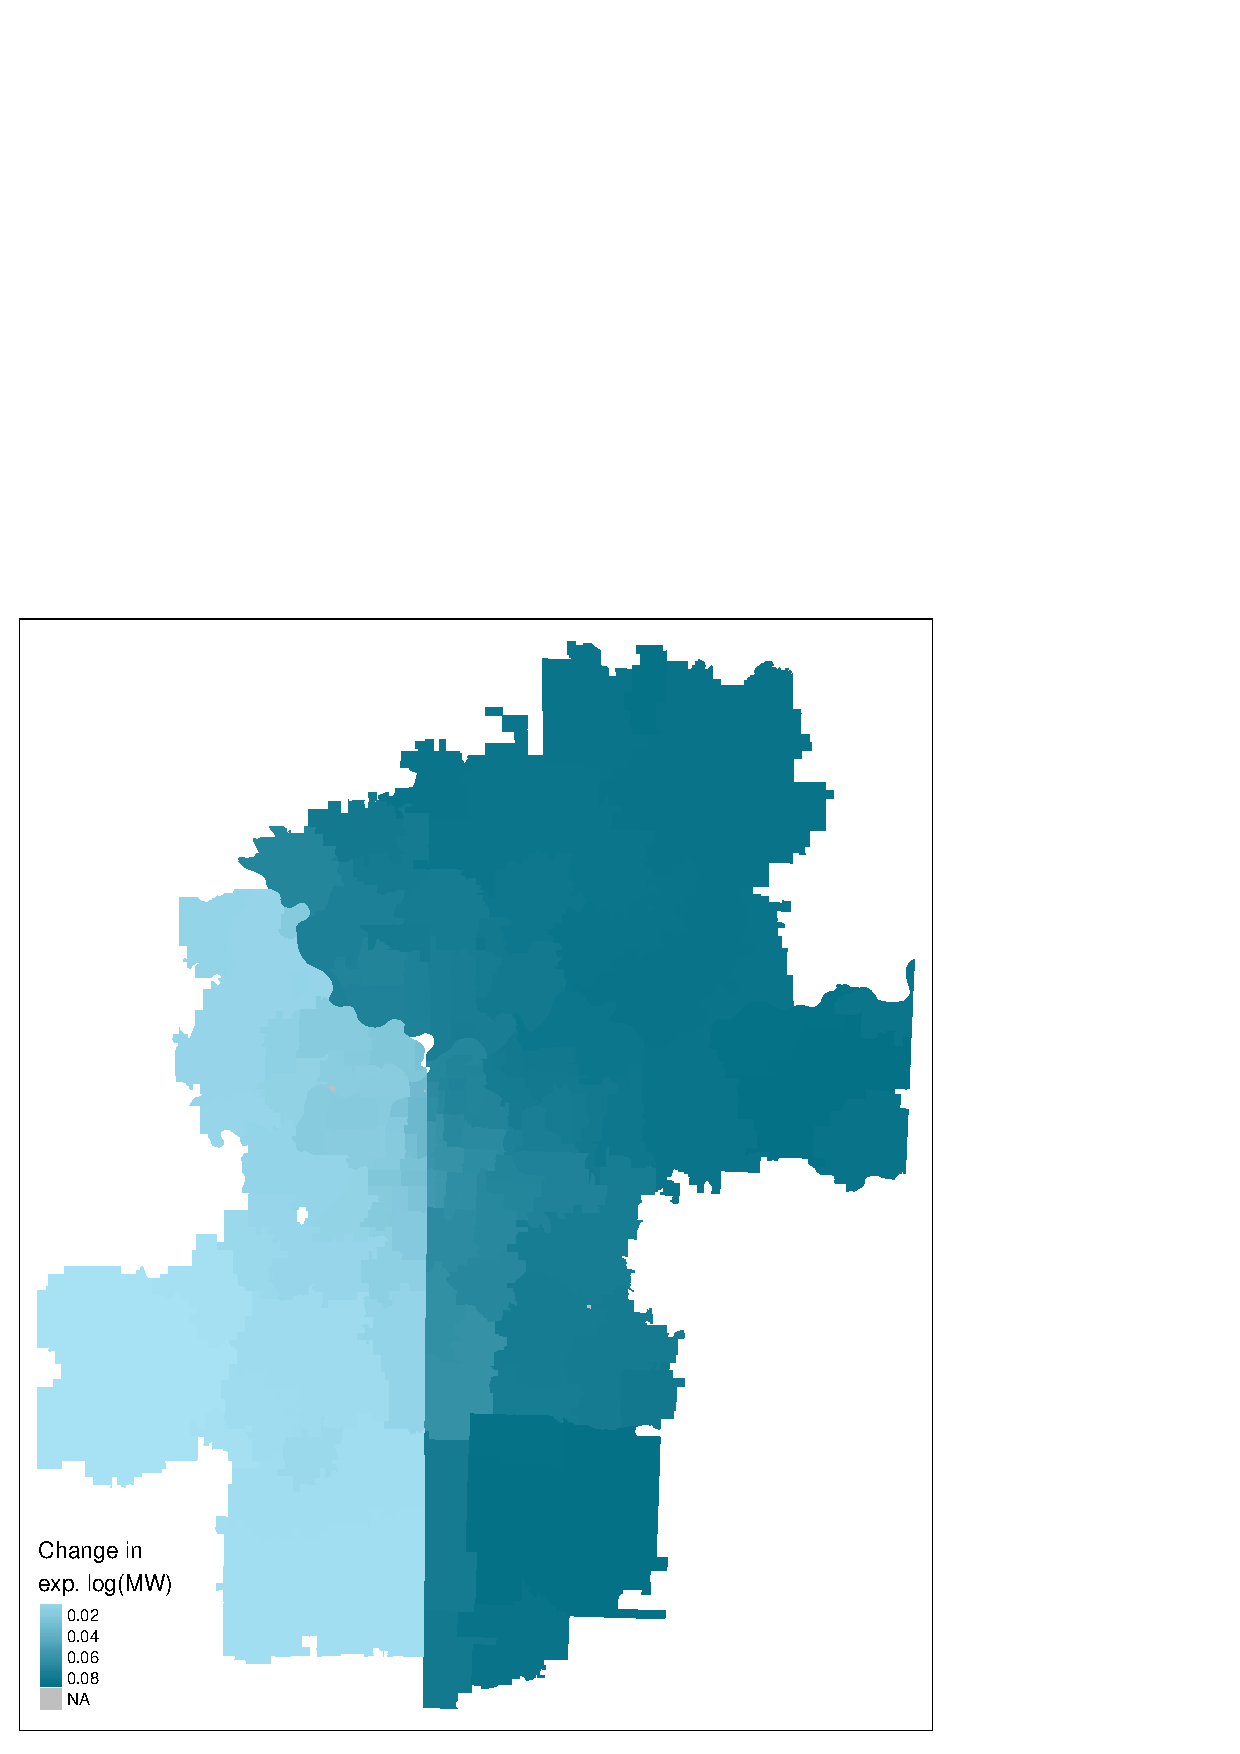
\includegraphics[scale = 0.36]{maps_events/output/kc2018-12_exp_mw.png}
            \end{figure}   
        \end{column}
    \end{columns}
\end{frame}

\begin{frame}
\frametitle{Other examples: New York (MW Changes in January 2019)}
    \begin{columns}
        \begin{column}{0.50\textwidth}
            \vspace{-4mm}
            \begin{figure}
                \centering
                \includegraphics[scale = 0.36]{maps_events/output/nyc_2018-12_actual_mw.png}
            \end{figure}   
        \end{column}
        \begin{column}{0.50\textwidth}
            \vspace{-4mm}
            \begin{figure}
                \centering
                \includegraphics[scale = 0.36]{maps_events/output/nyc2018-12_exp_mw.png}
            \end{figure}   
        \end{column}
    \end{columns}
\end{frame}

\begin{frame}
\frametitle{Other examples: Bay area (MW Changes in January 2019)}
    \begin{columns}
        \begin{column}{0.50\textwidth}
            \vspace{-4mm}
            \begin{figure}
                \centering
                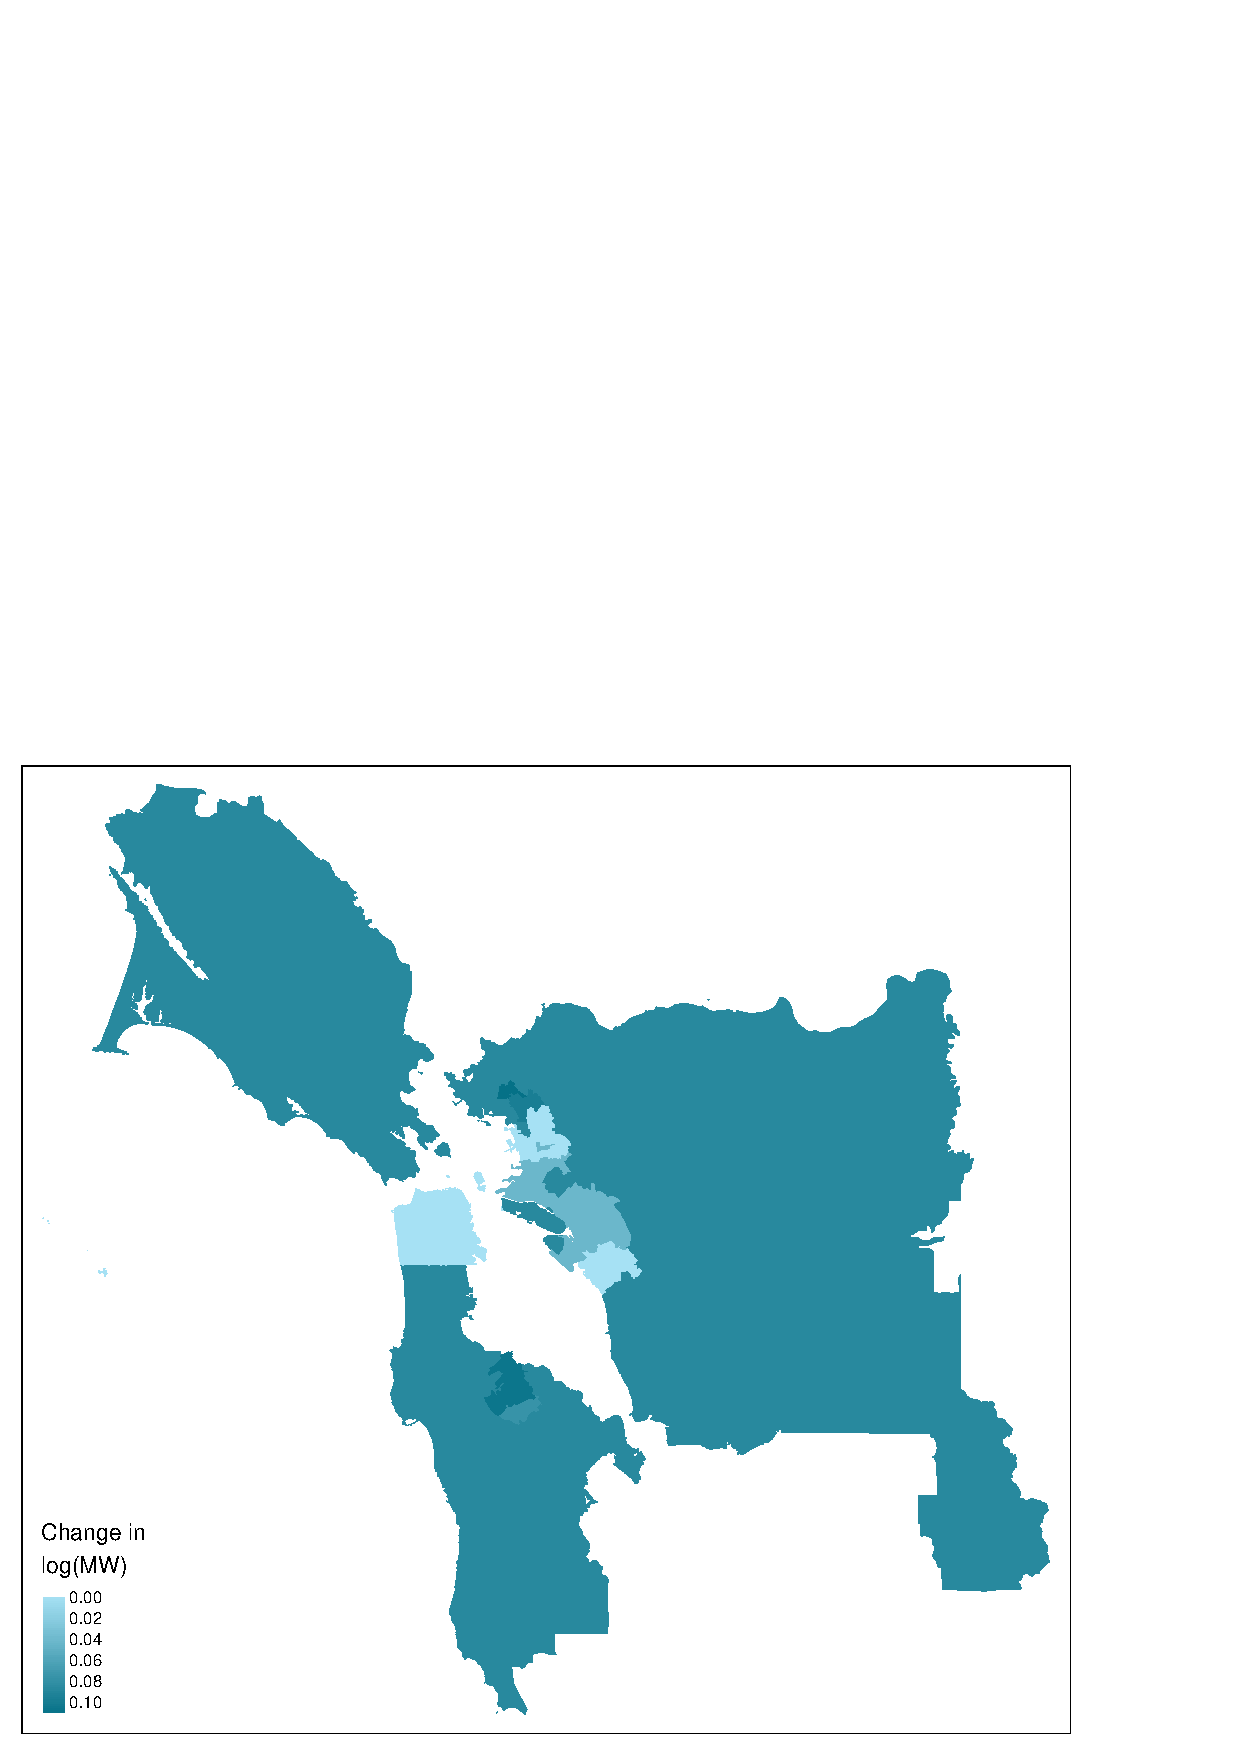
\includegraphics[scale = 0.36]{maps_events/output/bay_area_2018-12_actual_mw.png}
            \end{figure}   
        \end{column}
        \begin{column}{0.50\textwidth}
            \vspace{-4mm}
            \begin{figure}
                \centering
                
\includegraphics[scale = 0.36]{maps_events/output/bay_area2018-12_exp_mw.png}
            \end{figure}   
        \end{column}
    \end{columns}
\end{frame}

\begin{frame}
	\frametitle{Outline}
	\tableofcontents[hideallsubsections]
\end{frame}

\section{Model}

\section{Data}

%\subsection{Zillow}

\begin{frame}[label = zillow]
	\frametitle{Zillow Data}
	
	\begin{itemize}
		\item Leader online real estate and rental platform in the U.S. {\small (more 
		than 110 million homes and 170 million unique monthly users in 2019).}
		
		\vspace{2mm} \item
		Provides \textit{median} rents data at ZIP code, county, and state levels 
		at a monthly frequency for several housing categories.
		
		\pause
		\vspace{2mm} \item
		Use category single-family, condominium, and cooperative houses (SFCC):
		\begin{itemize}
			\item Most common housing type in the U.S.
			\item Most populated series in Zillow.
			%%\item Captures trends in metropolitan housing markets. 
			%%\hyperlink{zillow_safmr}{\beamerbutton{Comparison SAFMR}}
		\end{itemize}
		
		\pause
		\vspace{2mm} \item
		Limitation: Zillow sample is not random.
	\end{itemize}
\end{frame}

\begin{frame}
	\frametitle{Comparison between Zillow Sample and Population Density}
    \begin{figure}
    	\centering
    	\begin{subfigure}{0.46\textwidth}
    		\includegraphics[scale = 0.34]{maps_US/output/USPS_zipcodes_pop_density.png}
    	\end{subfigure}%
        \begin{subfigure}{0.46\textwidth}
        	\includegraphics[scale = 0.34]{maps_US/output/USPS_zipcodes_zillow_data.png}
        \end{subfigure}
    \end{figure}
\end{frame}

%\subsection{Minimum Wages}

\begin{frame}[label=stat_MW]
	\frametitle{The Statutory MW}
	
	\begin{itemize}
		\item
		Collect MW data at state, county and city levels between Jan 2010 and Dec 2019.
		
		\vspace{2mm} \item
		Assign those data to ZIP codes.
		
		\vspace{2mm} \item
		Define statutory MW in ZIP code as maximum between state and local levels.
		
		\pause
		\vspace{2mm} \item
		ZIP codes available in Zillow contain 18,689 changes at the ZIP code-month level.
		\vspace{-3.5mm} 
		\begin{itemize} \small
			\item 151 state-level changes.
			\item 182 county- and city-level changes.
		\end{itemize}
		%% We use 4,224 events at the ZIP code-month level in our estimating panel
		
	\end{itemize}
	
\end{frame}

\subsection{Commuting shares}

\begin{frame}
	\frametitle{Using LODES to construct the experienced log MW}
	
	Construct \textbf{origin-destination matrix} at ZIP code level from 2017 LODES.
	%% Original data comes at the block-group level
	Observe:
	\begin{itemize} \small
		\item Number of workers residing in a ZIP code and working in every other 
		ZIP code.
		\item Analogous, matrix for number of workers younger than 29 and earning less than 
		\$1,251.
		%% Exp MW constructed using any of these measures gives similar results
	\end{itemize}
\end{frame}

\subsection{Other Data sources}

\begin{frame}
	\frametitle{Other Data Sources} 
	
	\begin{itemize}
		\item Economic controls from the Quarterly Census of Employment and Wages 
		{\small (QCEW)}.
		\vspace{2mm}  \item IRS Statistics of income - ZIP Code Aggregates (New)
		\vspace{2mm} \item ZIP Code Month panel of rents since 2018 from actual transactions data (New)
	\end{itemize}
\end{frame}

\section{Empirical Strategy}

\subsection{Empirical Models}

\begin{frame}[label = stat_only_model]
	\frametitle{Empirical (Naive) model}
	
	Ignoring the experienced MW, one may estimate the following first differences model:
	
	$$
	\Delta \ln r_{it} = \tilde\delta_t + 
	\tilde\beta \Delta \ln \underline{w}_{it} + 
	\Delta \mathbf{X}^{'}_{c(i)t} \tilde\eta + 
	\Delta \tilde\varepsilon_{it} ,
	$$
	
	where	
	\begin{itemize} \small
	\item ZIP code $i$, county $c(i)$, month $t$;
	
	\item \vspace{1mm} $r_{it}$: rents per square foot;
	
	\item \vspace{1mm} $\ln \underline{w}_{it}$: statutory log MW;
	
	\item \vspace{1mm} $\tilde\delta_t$: month fixed effects (ZIP code FE $\tilde\alpha_i 
	$ is 
	implicit);
	
	\item \vspace{.5mm} $\mathbf{X}_{c(i)t}$: time-varying controls.
	\end{itemize}
\end{frame}

\begin{frame}
	\frametitle{Empirical model}
		
	Now add experienced MW:
	$$
	\Delta \ln r_{it} = \delta_t +
	    \beta {\color{red}\Delta \underline{w}^{\text{exp}}_{it}} +
		\gamma {\color{blue} \Delta \ln \underline{w}_{it}} + 
		\Delta \mathbf{X}^{'}_{c(i)t} \eta + 
		\Delta \varepsilon_{it} ,
	$$
	
	where $\underline{w}^{\text{exp}}_{it}$ is experienced log MW {\small (Recall 
	$\Delta \underline{w}^{\text{exp}}_{it} = \sum_{z \in \mathbb{Z}_i} \pi_{i z} \Delta 
	\ln \underline{w}_{zt}$)}.

	\pause
	\vspace{2mm}
	For causal effect of $\beta$ we need:
	$$
	E \left[\Delta \varepsilon_{ict} {\color{red} \Delta 
	\underline{w}^{\text{exp}}_{ic\tau}} 
	\big| {\color{blue}\Delta \ln \underline{w}_{ict}}, \delta_t, \Delta 
	\mathbf{X}_{ict} \right] = 0
	\quad \quad \forall \tau \in \left[ \underline{T}, \overline{T} \right]
	$$
	
	\pause
	\vspace{2mm}
	\textbf{In words}: conditional on FEs, controls, and {\color{blue} MW in same ZIP 
	code}, unobserved innovations to rent shocks are uncorrelated with past and future 
	values of log MW changes {\color{red} in nearby ZIP codes}.
\end{frame}


\begin{frame}
	\frametitle{Discussion Identification Assumption}
	
	Thus, for causal effect of $\beta$ we need:
	$$
	E \left[\Delta \varepsilon_{ict} \Delta \underline{w}^{\text{exp}}_{ict}  
	\big| \Delta \ln \underline{w}_{ict}, \delta_t, \Delta 
	\mathbf{X}_{ict} \right] = 0
	\quad \quad \forall \tau \in \left[ \underline{T}, \overline{T} \right]
	$$
	\vspace{.5mm}
	Analogously, for causal effect of $\gamma$ we need:
	$$
	E \left[\Delta \varepsilon_{ict} \Delta \ln \underline{w}_{ict}  
	\big| \Delta \underline{w}^{\text{exp}}_{ict}, \delta_t, \Delta \mathbf{X}_{ict} 
	\right] = 0
	\quad \quad \forall \tau \in \left[ \underline{T}, \overline{T} \right]
	$$
	
	\pause
	\vspace{.5mm}
	\textbf{Is this plausible?}
	\begin{itemize} \small
		\vspace{.5mm}
		\item MW policies are rarely set by considering differential dynamics of the 
		rental housing market within metropolitan areas.
		%% For example, the Congressional Budget Office (CBO) doesn't mention rents even 
		%% once in it's study of the effects of the Wage Act of 2021
		%% https://www.cbo.gov/system/files/2021-02/56975-Minimum-Wage.pdf
		
		\vspace{.5mm}
		\item Furthermore, there is substantial heterogeneity in the housing market 
		across ZIP codes.
		
		\vspace{.5mm}
		\item Indirectly test assumption through pre-trends, assuming no anticipatory 
		effects in housing market.
	\end{itemize}
\end{frame}

\begin{frame}[label = dyn_model]
	\frametitle{Testing Identification with a Dynamic model}
	
	Adding leads and lags of the experienced log MW:
	
	$$
	\Delta \ln r_{ict} = \delta_t
		+ \sum_{r=-s}^{s} \beta_r \Delta \underline{w}^{\text{exp}}_{ic,t+r}
		+ \gamma \Delta \ln \underline{w}_{ict}
		+ \Delta \mathbf{X}^{'}_{ct}\eta
		+ \Delta \varepsilon_{ict}
    $$
	
	where $\{\beta_r\}_{r=-s}^{s}$ are the dynamic coefficients.
	
	\vspace{1mm}

    Analogously, one can add instead the leads and lags of the log residence MW
    to test the identification assumption of $\gamma$.
\end{frame}

\section{Results}

\subsection{Main Results}

\begin{frame}
    \frametitle{Static }
    
\end{frame}

\begin{frame}
	\begin{figure}
		\centering
		\vspace{-2mm}
		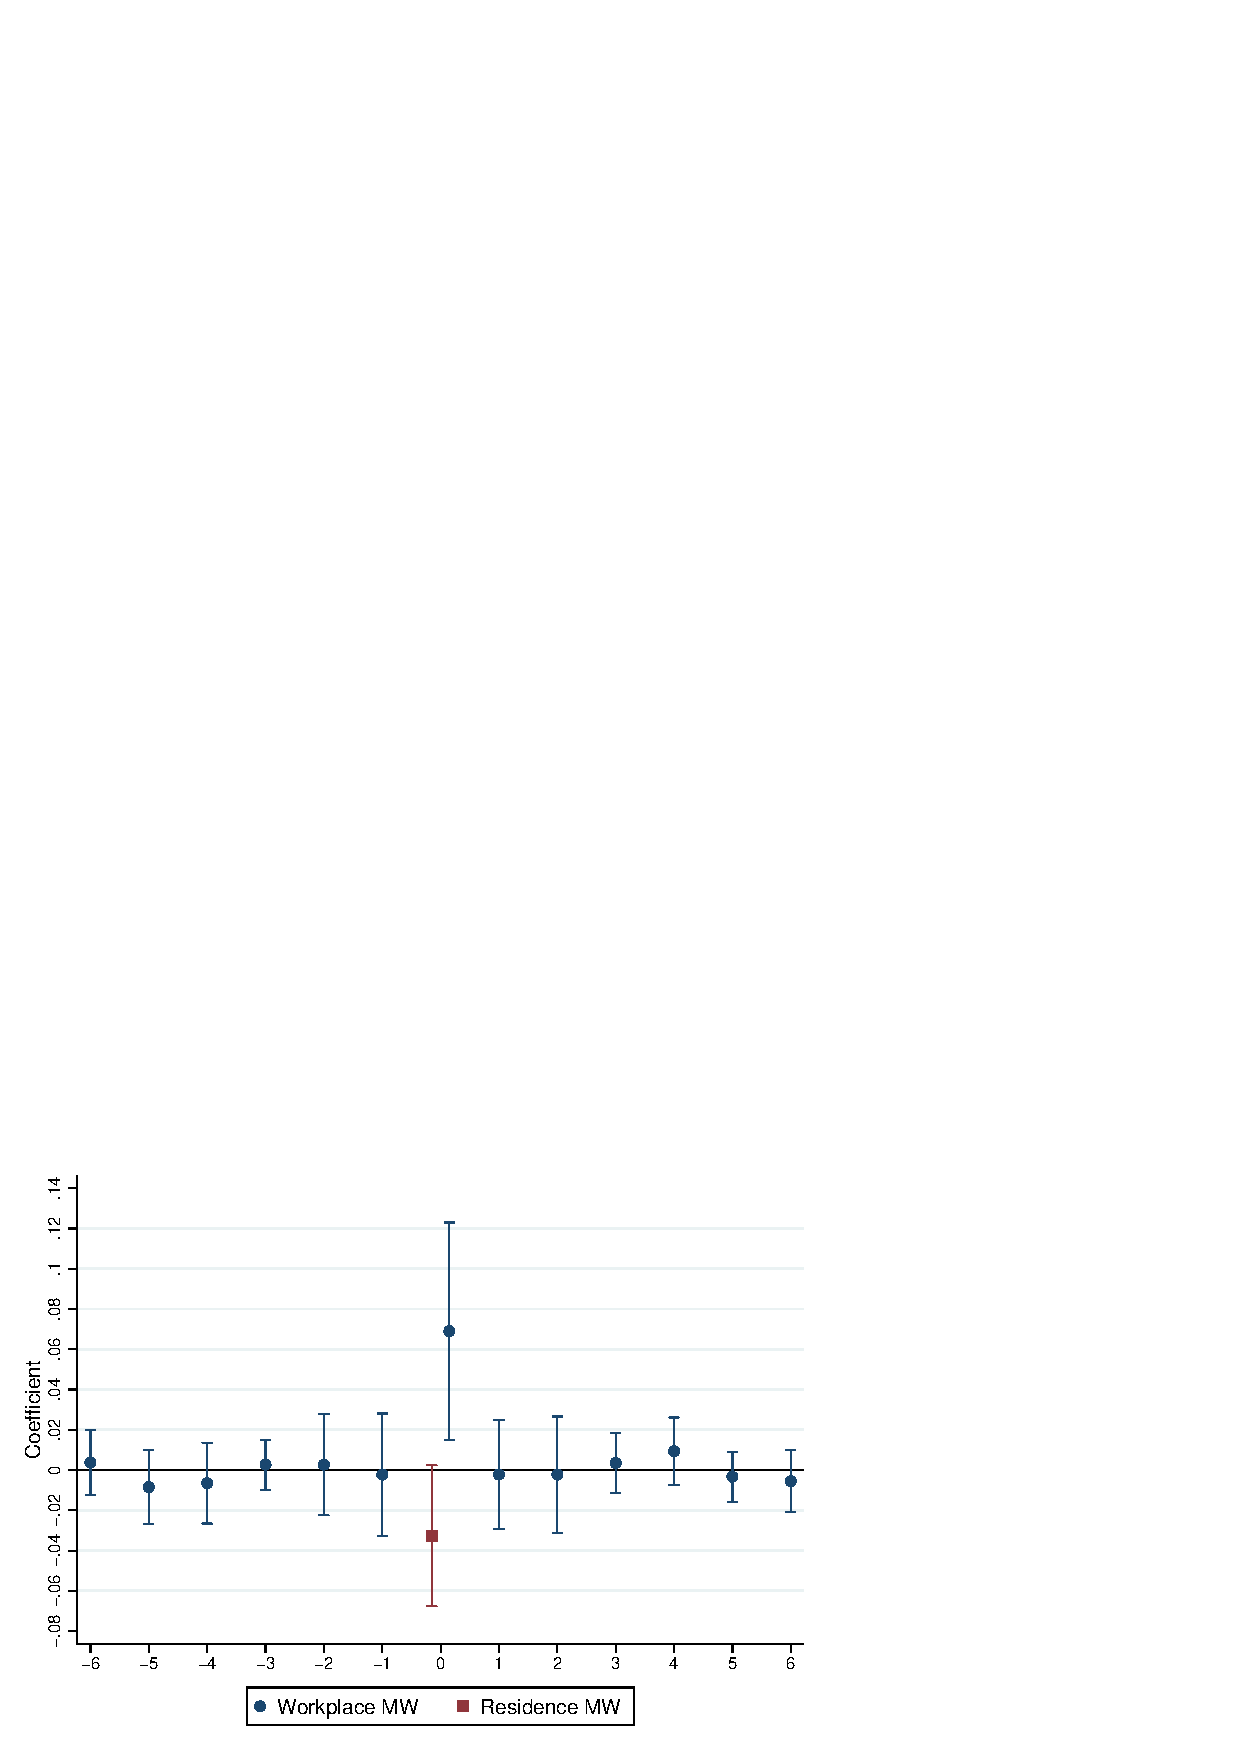
\includegraphics[width=0.8\textwidth]{fd_baseline/output/fd_baseline_exp_ln_mw_17_dynamic.png}
	\end{figure}   
\end{frame}


\section{Robustness}

\section{Heterogeneity}

\section{Counterfactuals}

\begin{frame}
    \frametitle{Objective}
    
    
    What is the share of the incremental wage bill generated by MW changes that ends up 
    in the pockets of landlords? 
    
    \pause
    
    Many interesting counterfactuals. Today, we will focus on a counterfactual increase of the 
    federal MW to \$9 in January 2020.
    
    \pause 
   
    Take $Y_z$ and $H_z$ as the total nominal income and total housing expenditure at Zip Code $z$. Let $h_z$ as  be the total square footage of rented housing. 
   
   Imagine there is a MW change that changes nominal income. We are interested in computing:
   
   \begin{equation}
   	    \rho = \frac{\Delta H_z}{\Delta Y_z} = \frac{h^{\text{Post}}_z r^{\text{Post}}_z - h^{\text{Pre}}_z r^{\text{Pre}}_z}{\Delta Y_z}
   \end{equation}
   
\end{frame}

\begin{frame}
    \frametitle{Counterfactuals - Total rented space}
    We don't observe $h^{\text{Pre}}_z$ and $h^{\text{Post}}_z $. We assume $h^{\text{Pre}}_z = h^{\text{Post}}_z = h_z$ so that:
    
    \[
    \rho = \frac{h^{\text{Post}}_z r^{\text{Post}}_z - h^{\text{Pre}}_z r^{\text{Pre}}_z }{\Delta Y_z} = h_z \frac{\Delta r_z}{\Delta Y_z}
    \]
   
   If $\Delta h_i = h^{\text{Post}}_z - h^{\text{Pre}}_z > 0$ then our estimate of $\rho$ is a lower bound.
\end{frame}

\begin{frame}
    \frametitle{Counterfactuals - Estimation}
    
    We will compute $\rho = h_z \frac{\Delta r_z}{\Delta Y_z}$ in 3 steps:
    \begin{itemize}
        \item \textbf{Step 1}: Get an estimate of $h_z$
        \item \textbf{Step 2}: Use our empirical model to compute $\Delta r_z$
        \item \textbf{Step 3}: Use an auxiliary model that maps MW changes to nominal income changes to compute $\Delta Y_z$
    \end{itemize}
    
    \pause
    
    \textbf{Step 1}
    
    Haven't found data on $h_z$. Therefore we do the following:
    
    \begin{itemize}
        \item In the Zillow data we observe the median rental price per square foot, $r_z$, but we also observe the median rental price, $R_z$.
        Therefore, we can compute $\frac{R_z}{r_z}$ and that gives us the square footage of the median rental at each Zip Code. Call it $q_z$.
        \item From the 2019 ACS, we get the number of households that are renting at in each ZIP Code. Call it $N_z$.
    \end{itemize}
    
    We take that:
    \[
    h_z = q_z N_z
    \]
\end{frame}

\begin{frame}
    \frametitle{Counterfactuals - Estimation}
    \textbf{Step 2}
    
    Pretend that the federal MW increase to \$9.
    \begin{enumerate}
        \item Compute the new binding MW in each Zip Code.
        \item Using the commuting shares and the new binding MW's compute the new experienced MW's in each ZIP Code.
        \item Compute $\Delta \ln r_z$ using our estimates.
        \item Compute $\Delta r_z = \exp(\Delta \ln r_z) r^{\text{Pre}}_z$, where $r^{\text{Pre}}_z$ is taken from the Zillow data at December 2019. 
    \end{enumerate}
\end{frame}

\begin{frame}
    Thanks!
\end{frame}

%%%%%%%%%%%%%%%%%%%%%%%%%%%%%%%%%%%%%%%%%%%%%%%%%%%%%%%%%%%%%%%%%%%%%%%%%%%%%%%%%%%%%%%%%%
%                                       APPENDIX                                        %
%%%%%%%%%%%%%%%%%%%%%%%%%%%%%%%%%%%%%%%%%%%%%%%%%%%%%%%%%%%%%%%%%%%%%%%%%%%%%%%%%%%%%%%%%%

\appendix

\renewcommand\thetable{\thesection.\arabic{table}} 
\renewcommand\thefigure{\thesection.\arabic{figure}} 
\setcounter{table}{0}
\setcounter{figure}{0}

\section{Appendix}


\end{document}
